\chapter{Implementazione}

\section{Linguaggi di programmazione}

Per la parte in esecuzione sui Raspberry Pi si è scelto di utilizzare Python 3 che garantisce un elevato supporto per i sensori e attuatori attualmente disponibili.

Il web server è stato implementato utilizzando HTML5, CSS e JavaScript.

Il server //TODO

\section{Protocolli di comunicazione}

REST+TCP+TLS

\section{Criticità}

Criticità nel normale esercizio del sistema, come la disconnessione di un Raspberry dalla rete, sovraccarico del server, led si fulmina (teoricamente è possibile accorgersene? Se no, lo togliamo).

\section{Implementazione della parte embedded}

\subsection{Configurazione dei Raspberry Pi}

Si è scelto di installare su ogni Raspberry la distribuzione Linux Raspbian perché attualmente è l'unica ufficialmente supportata.
In ogni caso installando Python e tutte le dipendenze necessarie al progetto, sarebbe possibile utilizzare anche una qualsiasi altra distribuzione Linux.

I messaggi che i Raspberry Pi inviano quando comunicano con il server contengono al loro interno anche un timestamp per fini statistici.
Per evitare che con il tempo l'ora vada fuori sincrono si è impostato l'aggiornamento con \textit{ntp} giornalmente invece che, come di default, ad ogni avvio.
Questo perché i Raspberry Pi una volta dislocati sul territorio rimarranno sempre accesi senza effettuare mai riavvii a meno che non si presentino dei problemi.


\subsection{Paradigma ad attori e organizzazione a task}

Dato che il software dei Raspberry è composto da diverse parti tra loro autonome, si è scelto di adottare il paradigma ad attori.
In questo modo ogni sottoparte è un attore e la comunicazione avviene tramite scambio di messaggi.
A tale scopo si è utilizzata la libreria \textit{pykka}.

Come visto in fase di progettazione, i Raspberry devono poter eseguire diverse operazioni concorrentemente.
Per questo motivo è stata utilizzata la libreria \textit{threading} di Python che permette ad un singolo programma l'esecuzione di più thread.

\subsection{Controllo presenza auto \label{cpa}}

Per controllare la presenza di auto sulla carreggiata viene effettuato il calcolo della distanza utilizzando il sensore ad ultrasuoni HC-SR04. Per mitigare eventuali errori grossolani nella misurazione vengono effettuate sempre due misurazioni calcolando successivamente la media.

Il thread che si occupa del sensore di prossimità utilizza un secondo thread per inviare il segnale ad ultrasuoni.
Grazie a questa scelta si evita che il thread principale del sensore vada in busy waiting attendendo l'invio e il ritorno del segnale ad ultrasuoni.

Inoltre si è utilizzata la funzione \textit{wait\_for\_edge} che permette di fermare l'esecuzione del thread fino a quando non viene rilevata un'oscillazione, consumando una quantità irrisoria di CPU.

Il processo di controllo presenza auto è rappresentato da un attore il quale, dopo aver effettuato un controllo, notifica tutti i lampioni interessati.

\newpage
\lstinputlisting{code/ultrasonic.py}

\subsection{Rilevamento intensità luminosa}

Considerando che il Raspberry Pi non dispone di PIN analogici, per effettuare le letture di luminosità è possibile utilizzare una fotoresistenza analogica passando per un \textit{analog to digital converter (ADC)} oppure utilizzare direttamente un sensore di luminosità digitale.

In questo progetto si è optato per la seconda opzione utilizzando il sensore digitale TSL2561.

Come per il controllo presenza auto della sezione \ref{cpa}, anche il processo di rilevamento è rappresentato da un attore.


\subsection{Scheduling illuminazione \label{si}}

Per consentire agli addetti ai lavori una programmazione agevole di ogni singolo lampione si è scelto di permettere la loro modifica sia tramite interfaccia web che tramite file di testo.

Per questo le impostazioni vengono salvate su file con estensione \textit{"cfg"} con una sintassi che permette la lettura e modifica anche manuale.

Grazie a questo comportamento si rende possibile sia la modifica dello scheduling di un singolo lampione con la comodità della interfaccia web, sia una modifica più avanzata collegandosi per esempio in SSH ad un Raspberry e cambiando i valori manualmente sui file di configurazione.

\lstinputlisting{code/light0.cfg}
\newpage

\subsection{API REST}

Come scritto in fase di progettazione, i Raspberry Pi devono esporre un insieme di API di tipo REST per permettere di modificare le impostazioni relative alla programmazione dei lampioni.
Per tale scopo è stato utilizzata la libreria \textit{Flask}.

Quando un Raspberry riceve una richiesta tramite le API, per prima cosa vengono controllate le credenziali fornite perché è sempre richiesta una autenticazione tramite username e password per poter effettuare una qualsiasi GET o POST.

Se la richiesta ricevuta è valida, verrà restituito un json, o con i dati richiesti o semplicemente con il codice 200, se la richiesta non prevedeva dati di ritorno.

\section{Implementazione del Web Server REST}

Come scritto nella sezione \ref{si} per permettere agli addetti ai lavori di controllare e modificare la programmazione dei singoli lampioni è stata implementata una interfaccia Web tramite un server REST.

Come misura di sicurezza, tutte le richieste GET e POST ai Raspberry dovranno essere corredate da nome utente e password relativi al singolo dispositivo embedded che si intende contattare (mmm, la storia del "dare ad un addetto solo le credenziali dei rpi della sua zona dove lo mettiamo?).

Il sito Web è stato realizzato seguendo uno stile minimale, moderno e il quanto più intuitivo per l'utente.
L'interfaccia è ottimizzata sia per un uso desktop che mobile.

\begin{figure}[tbp]
	\centering
	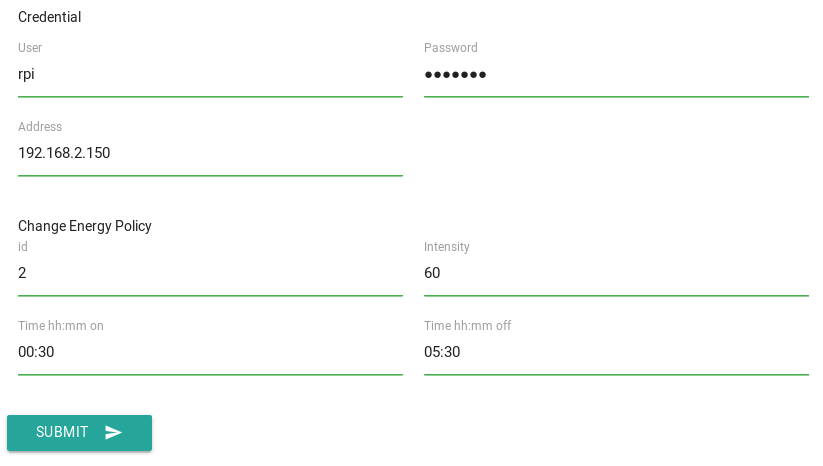
\includegraphics[scale=.62]{figure/web_desktop.png}
	\caption{Interfaccia web Desktop \label{FSM POLICY}}
	\subfloat[(Mobile) Campi corretti]{{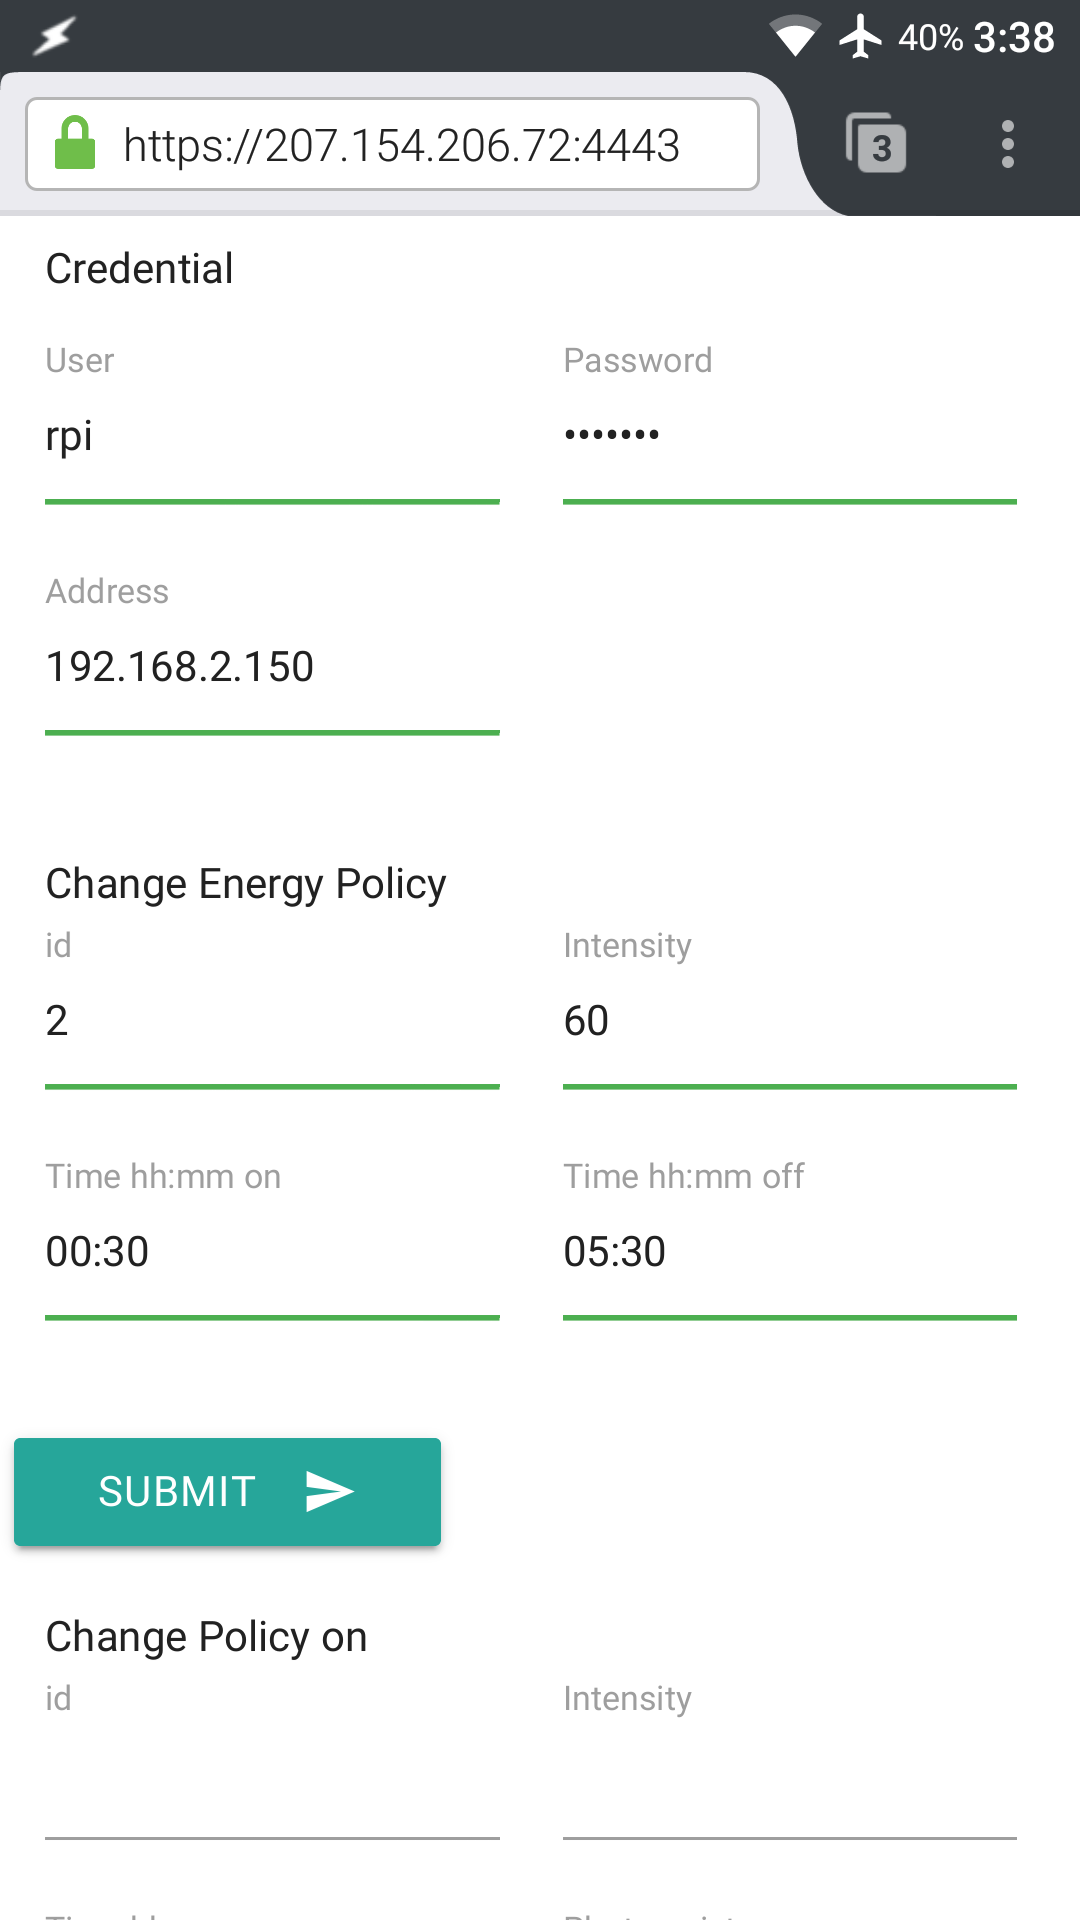
\includegraphics[width=6cm]{figure/web_mobile.png} }}%
	\qquad
	\subfloat[(Mobile) Campi mancanti o errati]{{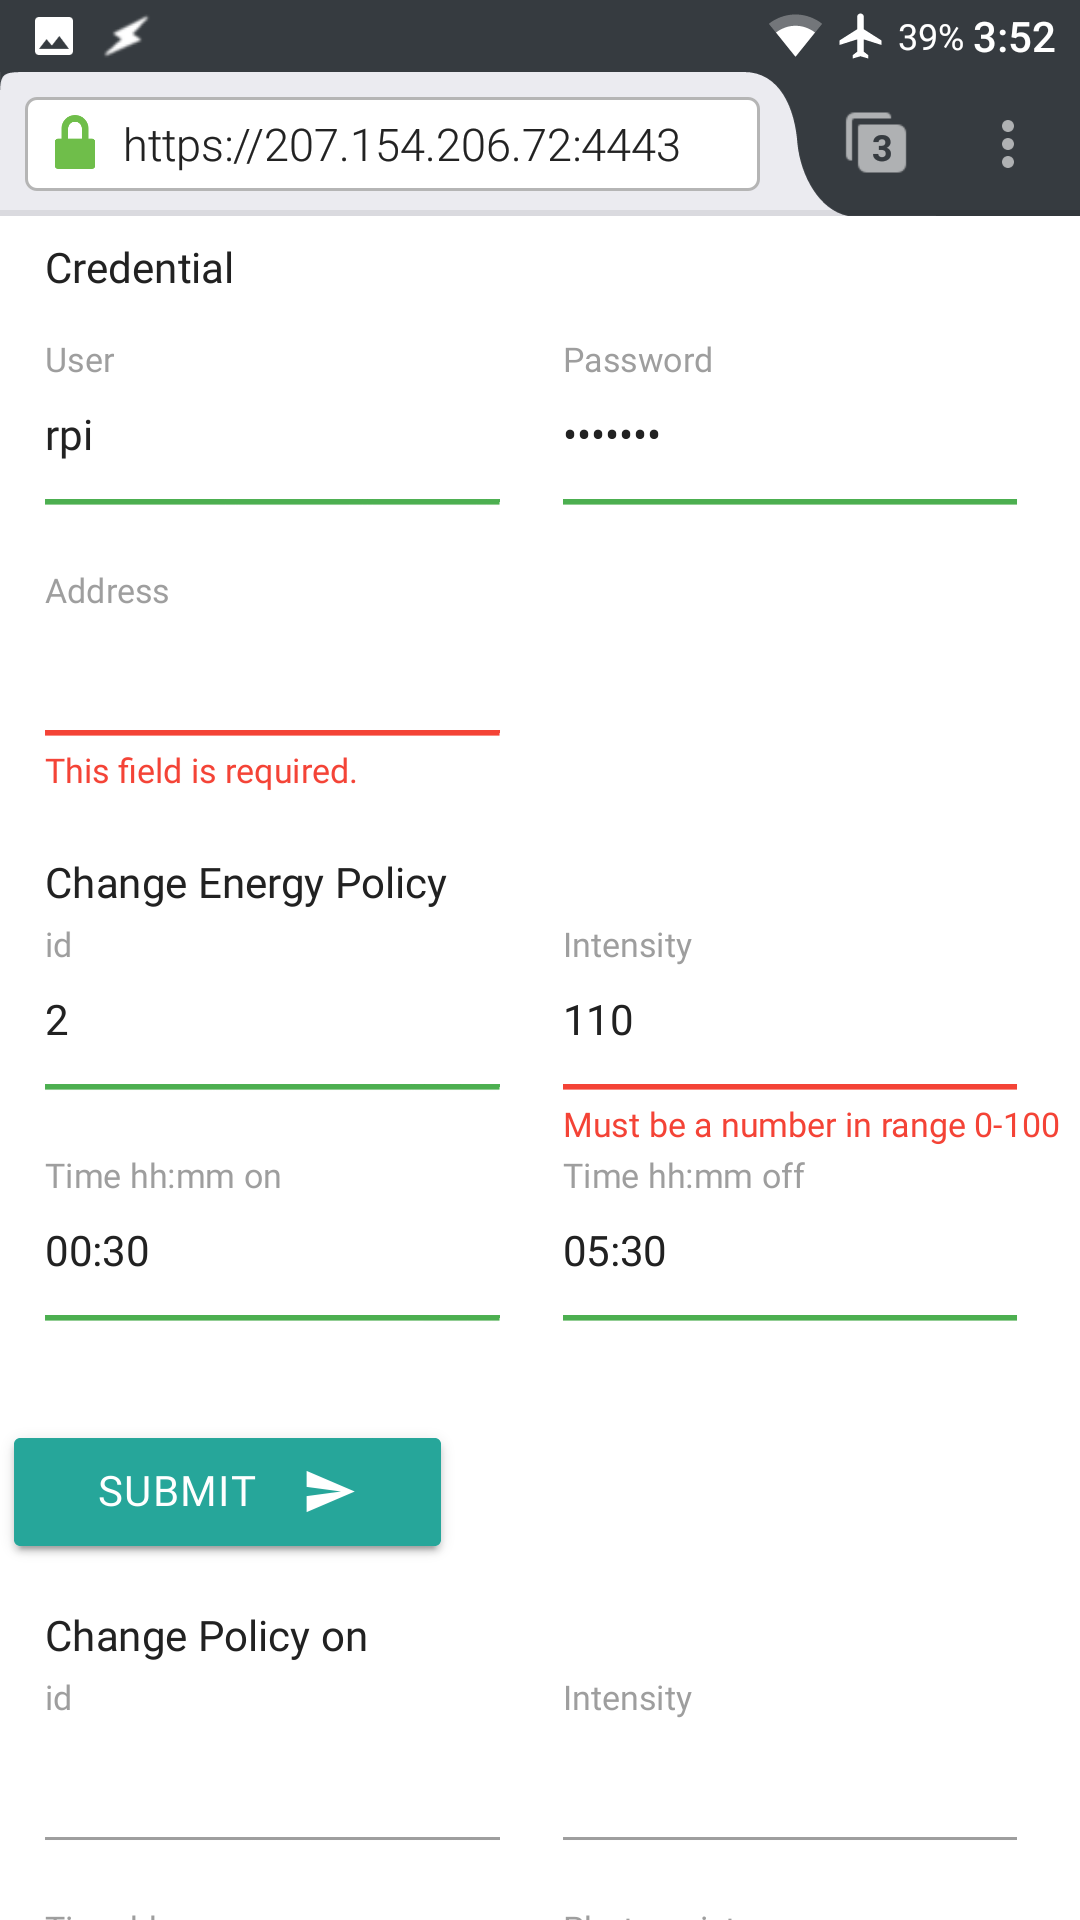
\includegraphics[width=6cm]{figure/web_mobile_errors.png} }}%
	%\caption{Esempi della interfaccia mobile}%
	\label{fig:example}%
\end{figure}

\newpage

\subsection{Linguaggi e librerie}

Il Web Server è stato realizzato utilizzando i linguaggi HTML, CSS e JavaScript.

Per il CSS si è utilizzata la libreria \textit{materialize}, mentre per quanto riguarda JavaScript si è utilizzato \textit{JQuery} e \textit{JQuery validate} per effettuare controlli client side sui form compilati dagli utenti.

\subsection{Modalità Debug}

Per permettere agli addetti ai lavori di effettuare controlli sui lampioni, come per esempio verificare il loro corretto funzionamento, è stata prevista la possibilità di abilitare la modalità debug.

Entrando in modalità debug i lampioni si accenderanno e spegneranno in base ai comandi che verranno impartiti manualmente dagli addetti e ignoreranno le eventuali policy impostate in precedenza.
